\section{Development and testing}

\subsection{Range tests}

One of the most important tests to carry out prior to deployment in the field
was testing the range of the devices.

In this experiment I took four challenger RP2040s to The Downs, a large public
park in Bristol. Here I tested four different antenna configurations to compare
how well the signal travelled across an increasing distance. Signal strength can
be measured using the received signal strength index (RSSI), a measure of the
difference in signal from the transmitter to the receiver and measured in
decibels (CHECK THIS).

For the test, two challengers were programmed as transmitters, sending an
example data packet similar to the data that would eventually be used at the
farm. One of the transmitters used a simple PCB antenna
(Figure~\ref{fig:pcb-antenna}) while the other used a higher range whip style
antenna (Figure~\ref{fig:good-antenna}). Then I programmed two challengers as
receivers, again one had a low range antenna and the other a long range one.

This meant that four different antenna configurations could be tested
concurrently, as the receivers could pick up the signal from each transmitter.
An estimate of their estimated relative performance before testing is shown
below:

\begin{enumerate}
    \item Whip antenna to whip antenna (Likely best result)
    \item PCB antenna to whip antenna
    \item Whip antenna to PCB antenna
    \item PCB antenna to PCB antenna (Likely poorest result)
\end{enumerate}

The reason PCB transmitter to whip receiver will likely outperform the whip to
PCB configuration is that generally it is more important that the receiver has
better "hearing" capabilities than the transmitter can "shout".

Nine different distances from transmitter to receiver were tested, in 200m
increments starting from 0m as a baseline to a distance of 1600m
(Figure~\ref{fig:range-test-markers}). An important aspect in getting a
successful LoRa connection is whether there is line of sight between the
transmitter and receiver. Figure~\ref{fig:range-test-elevation} shows the
elevation profile of the test area, with the initial large dip being an
inaccuracy from google earth's topology data as the 0m point is near a cliff
edge. The lowest elevation point is at the starting point at around 83m above
sea level, while the highest point was at the 1km mark at around 94m making an
elevation range of 11m. My hypothesis was that signal would likely drop off or
stop entirely beyond this point as points beyond 1000m would be below the hill
line. This would effectively mean that the receivers would be in a signal shadow
point where the transmission waves would not be able to reach them. The only
possibility for signal to reach this area would be from reflections either from
nearby buildings or topology. However the effects of reflections are virtually
impossible to account for in the real world and therefore no accurate
predictions could be made.

\begin{figure}[H]
    \centering
    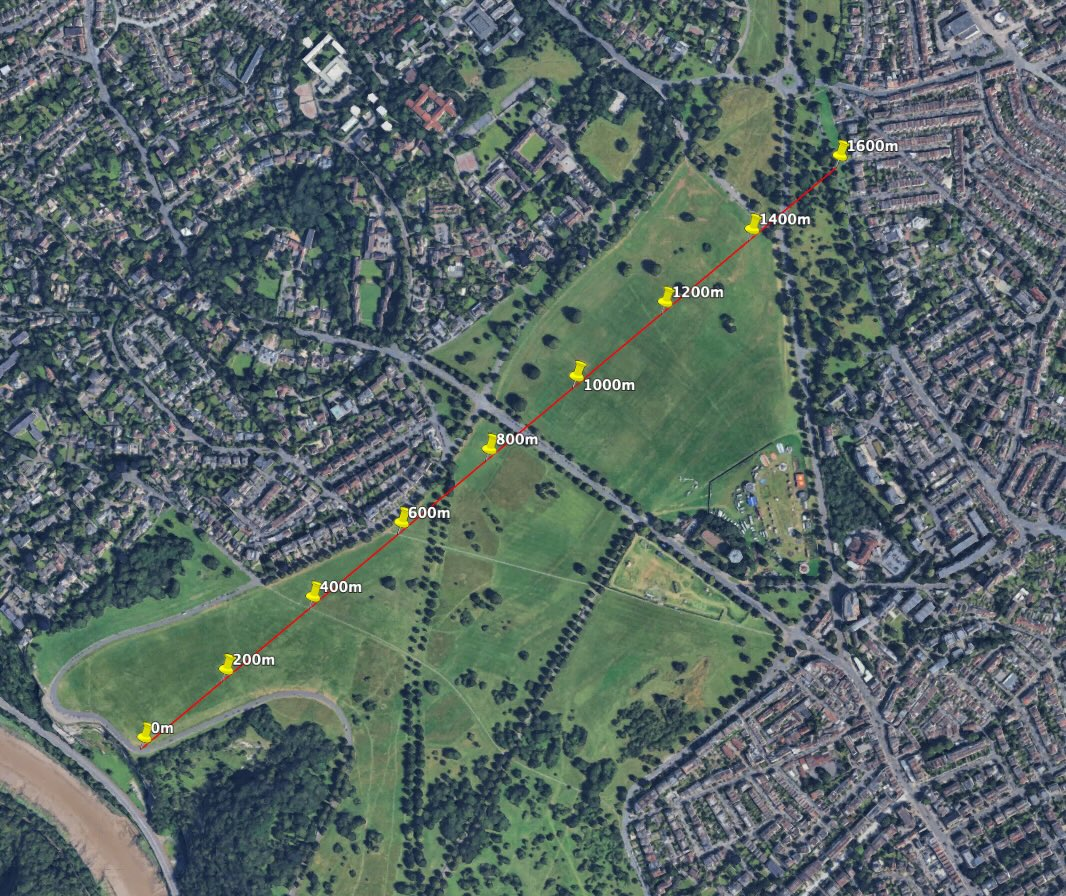
\includegraphics[width=0.8\textwidth]{contents/part-2/fig2/range-test-markers.jpg}
    \caption{Google earth image of data collection points}
    \label{fig:range-test-markers}
\end{figure}


\begin{figure}[H]
    \centering
    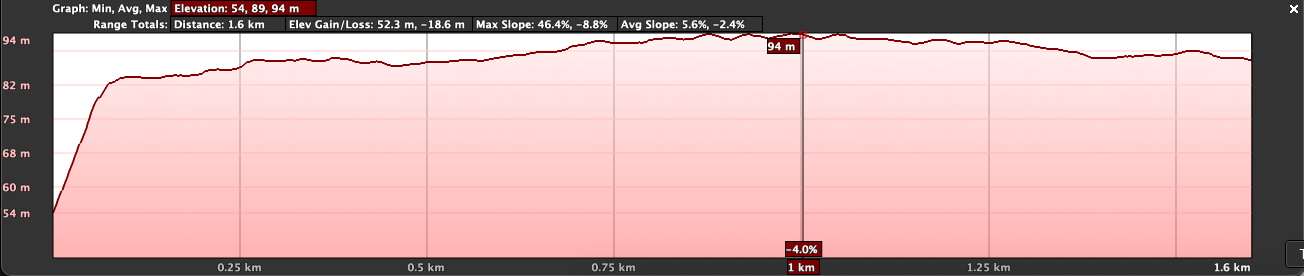
\includegraphics[width=1\textwidth]{contents/part-2/fig2/range-test-elevation-profile.jpg}
    \caption{Elevation profile of test area (ignore large dip at start)}
    \label{fig:range-test-elevation}
\end{figure}

At the time of the actual test however a festival was being run between the
1200m and 1400m mark. The festival had a number of large tents and temporary
buildings constructed which almost certainly blocked the signal. Therefore tests
past this point should be heavily caveated. It is likely this contributed to the
lack of signal past this point. Final data below:

\begin{figure}[H]
    \centering
    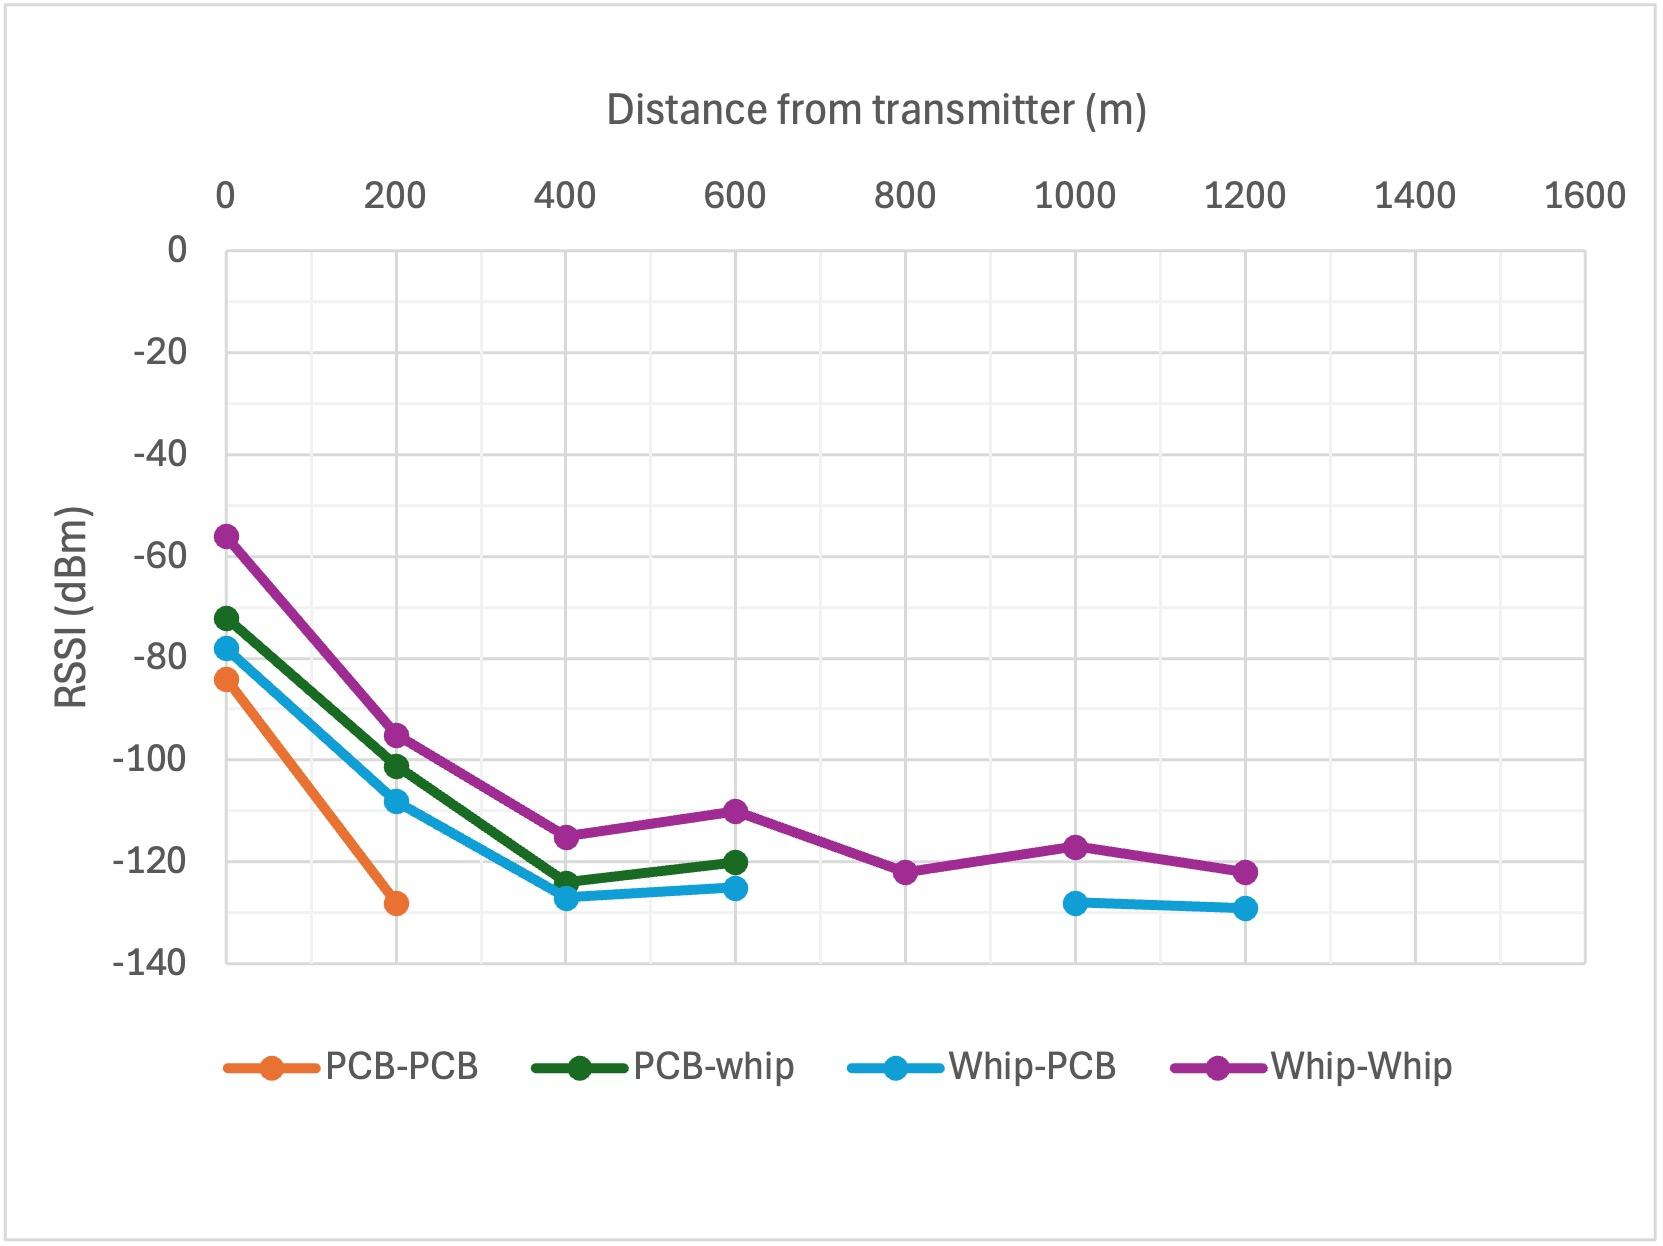
\includegraphics[width=1\textwidth]{contents/part-2/fig2/distance-graph.jpg}
    \caption{Graph to show signal loss from different receiver and transmitter configurations (higher is better)}
    \label{fig:range-test-graph}
\end{figure}

\subsection{Battery tests}

There is no mains electricity available in the apple field so the nodes must be
able to operate without external power source. Even with the use of a solar
panel the node must be able to work through the night and during periods of
dense cloud coverage where the solar panel will not have sufficient power to
keep the node running. This is where the use of a battery is particularly useful
as the solar panel can charge the battery with excess energy during periods of
excess solar radiation, such as during midday hours, and then store this energy
for periods of low or no solar radiation.

However, while daylight will be of little concern during the summer months when
this dissertation is being written, there will be far fewer days of usable
sunlight over the winter period. As the UK has very high latitude, there is
large seasonal variation in the length of a day. For the town of crediton
(nearest town to \farmName), in the summer there are 16.5 hours of daylight
while in winter it receives only 7.6 hours; meaning a night that is 16.4 hours
long. Therefore the node must have a battery sufficiently large to power it for
a minimum of 16.4 hours with some additional charge to account for high cloud
cover during the early evening and morning period.

To see if the battery solution was sufficient for this environment a test was
run on a fully charged 18650 battery that was then connected to the solar power
manager to allow the voltage to be regulated up to the challenger's 5v input
voltage.

A digital multimeter was installed between the solar power manager and the
challenger's usb c input to view the voltage and current in real time as well as
running a timer for the test and a calculation of the number of watt-hours
consumed by the node. The node was then run with a full suite of sensors
attached. During the test the node used 80ma at 5V for a wattage of 0.4W.

The node ran until the battery would no longer discharge, with the final battery
life of the node being 19 hours and 17 minutes. The meter showed that the node
consumed 7.96Wh of power. Considering the battery capacity is 9 Wh it may seem
that the battery ran out too quickly. However, the solar power manager
documentation tells us that the battery boost efficiency - being the conversion
of battery voltage from native 3.7V to 5V output - is only 86\%. With that in
mind effective battery capacity is roughly 7.74Wh, which is very similar to the
actual result.

The achieved result of 19 hours should be sufficient for running the node
continuously for much of the year as this compares to the longest night period
of 16.4 hours. However, during periods of heavy cloud cover in winter there is a
chance the node would not be able to charge the battery sufficiently in the day
to allow the node to run over night.

\subsection{Solar panel testing}

The solar panel is rated for 6W maximum power. This however would only
realistically be achieved under optimal conditions with a clear sky and full sun
around midday. This power rating was first verified using a multimeter on such a
day where a voltage of (INSERT VOLTAGE) and amperage of (INSERT AMPERAGE) was
measured for a wattage of (INSERT WATTAGE).

As explained in the battery section above, the node consumed about 7.96wH over a
19 hour and 17 minute period. We can therefore determine that the node requires
roughly 10wH of energy per day to able to run continuously. It would be tempting
to then say that the node would need less 2 hours of ideal sunlight to operate
for an entire day (being 6W * 2h = 12Wh), however we must also account for the
energy loss when converting from raw solar output to regulated 5V input that
challenger accepts.

The solar panel manager rates it's conversion efficiency for solar at 78\%
meaning for each watt of solar energy received 22\% of this will be wasted as
heat when converted to the correct voltage. If we adjust for this loss we would
need effectively 12.8Wh of energy just to power the node for a day, being 2
hours and 8 minutes of ideal conditions.

An additional 9Wh is needed to charge the battery which if we adjust again for
solar efficiency factor we get 11.5Wh. This is an additional 1h:55m of ideal
sun, leaving a total sunlight requirement each day of 4h:03m.

\subsection{Hardware assembly and weatherproofing}

Since most of the hardware in this project contains exposed electronics, the
final assembled devices needed to be made wind and water resistant to prevent
failure. However the sensors and solar panel would also need to be exposed to
perform their function effectively - e.g. a solar panel must have a clear view
of the sun throughout the day. The final design therefore needed to balance
multiple conflicting purposes:

\begin{itemize}
    \item The core electronics (challenger, solar manager, battery etc) must be
          kept dry, cool and away from wind which may damage electronics.
    \item The wind sensor must be exposed to the elements and securely fastened
          to withstand intense wind, it must also be kept high off the ground
          for more accurate readings.
    \item The solar panel must be exposed to the elements and be south facing at
          at an angle of 30-40 degrees to optimise solar efficiency.
    \item The soil moisture sensor must be inserted into the ground and as it
          has exposed electronics must be made waterproof.
    \item The antenna of the challenger must be placed as high as possible (at
          least 1.5m from the ground).
    \item The temperature/humidity sensor must be exposed to the elements to
          ensure accurate readings but cannot be exposed to rain due to the
          exposed electronics on it.
\end{itemize}

Due to the conflicting nature of some of these needs. The final device would
need to allow for positioning of different components at different heights.

The final design therefore was to place most of the sensitive electronics inside
a waterproof box with cut-outs for the to allow for external component wires.
This could then be mounted onto a 2m pole to allow for a good antenna signal and
more accurate wind speed readings.

\subsubsection{Sensitive electronics}

An IP65 waterproof junction box was selected to house the non-sensor portion of
the electronics. An IP rating measures the Ingress Protection of a devices
housing against water and dust defined by the International Electrotechnical
Commission. The first number of an IP code is a measure of dust resistance while
the second number is a measure of water resistance. An IP code of 65 therefore
means the box used here has perfect dust resistance and can withstand water jets
being sprayed at it from multiple directions \cite{wiki-ip}. This level of
protection should be more than adequate to withstand the heavy rainfall it will
experience.

\begin{figure}[H]
    \centering
    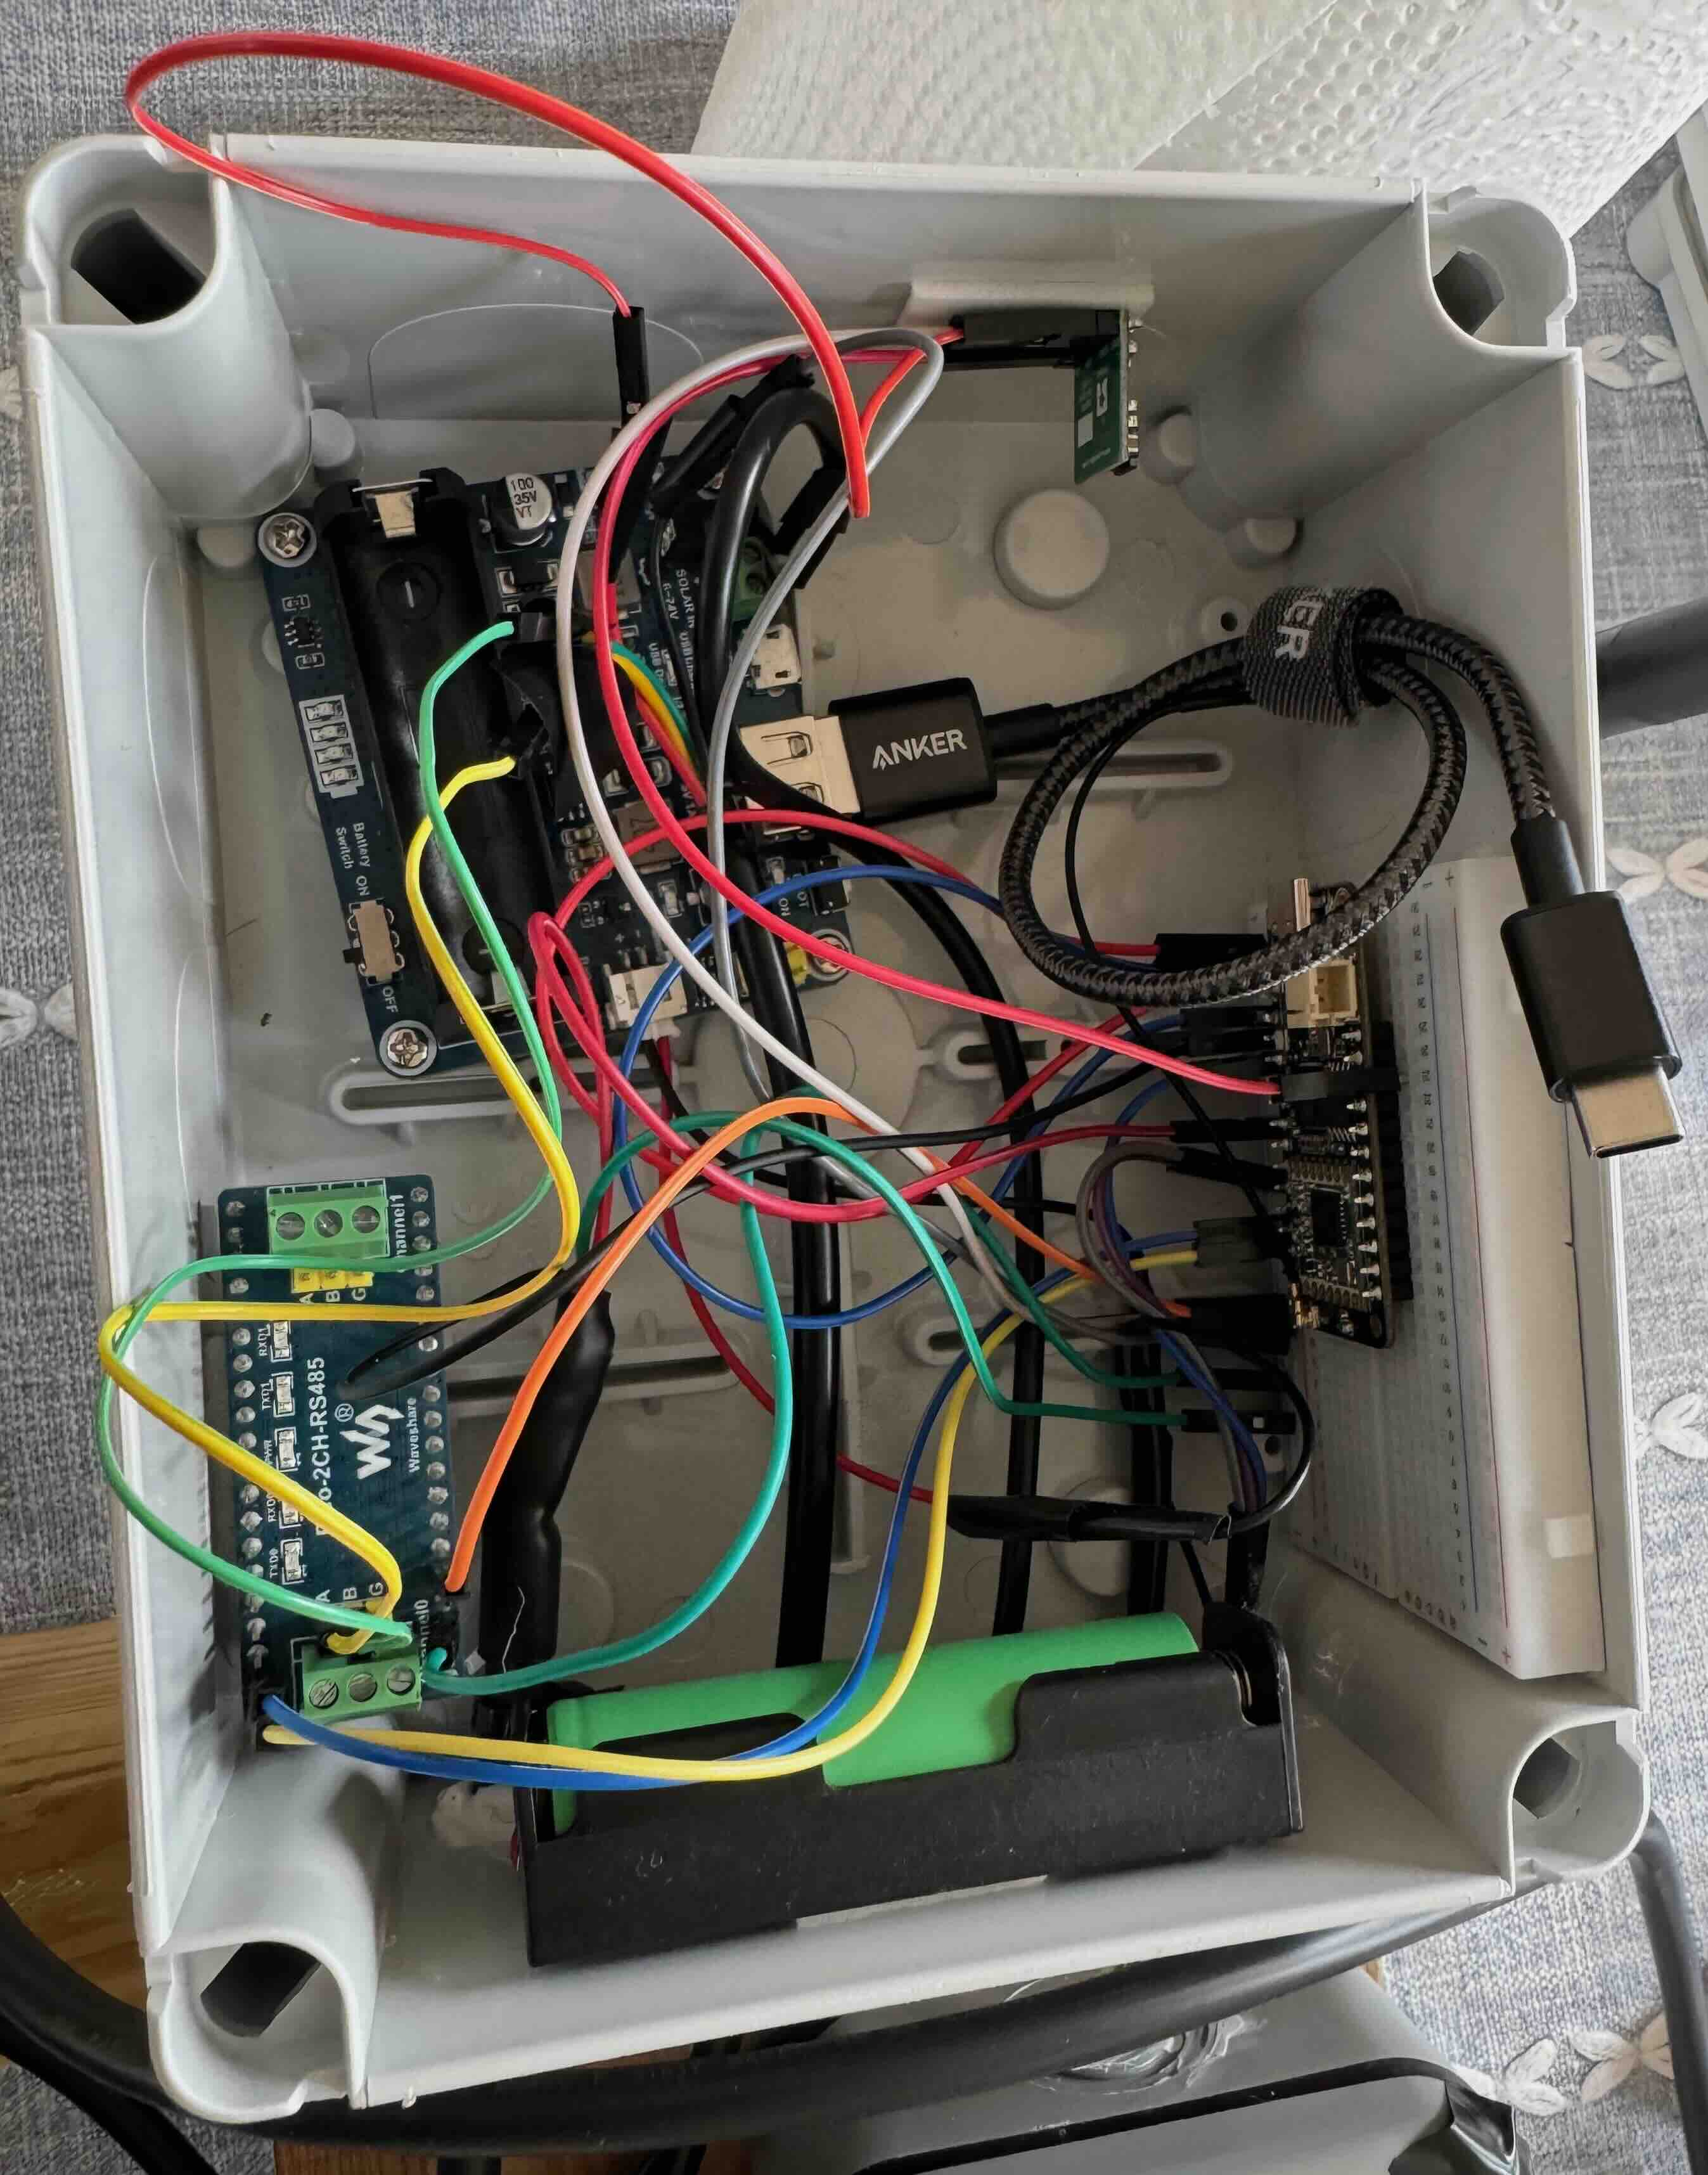
\includegraphics[width=0.5\textwidth]{contents/part-2/fig2/box-internals.jpeg}
    \caption{Open junction box showing internal wiring}
    \label{fig:box-internals}
\end{figure}

The challenger microcontroller was inserted onto a half size breadboard and then
stuck to one side of the box. The antenna cable was routed to the top right
corner where a small hole was drilled to allow for the antenna to be mounted
externally. All the other components were then wired into the breadboard and
stuck down with double sided sticky pads to prevent damage during transport or
heavy winds. The bottom of the box then had holes drilled for the anemometer,
soil moisture sensor, solar panel and temperature/humidity sensor respectively.
To prevent water ingress into these holes, sealant was deposited over the holes.

The entire box was then attached to a plank of wood measuring roughly 25cm by
60cm. This board holds all the sensors with the exception of the soil moisture
sensor which must be able to hang freely.

\subsubsection{Soil moisture sensor}

The sensor that required the most thought into waterproofing and mounting was
the capacitative moisture sensor. The first challenge was the need for the soil
moisture sensor to be able to reach ground level while at the same time the
microcontroller collecting it's readings was secured 2m above it. The solution
to this was to swap the small included wires with a 2.5m weatherproof cable
containing three cores (one for power, one for ground and one for data). Each
cable core was then soldered onto the sensor as in figure
~\ref{fig:solder-soil}, allowing for the sensor to be inserted into the ground.

\begin{figure}[H]
    \centering
    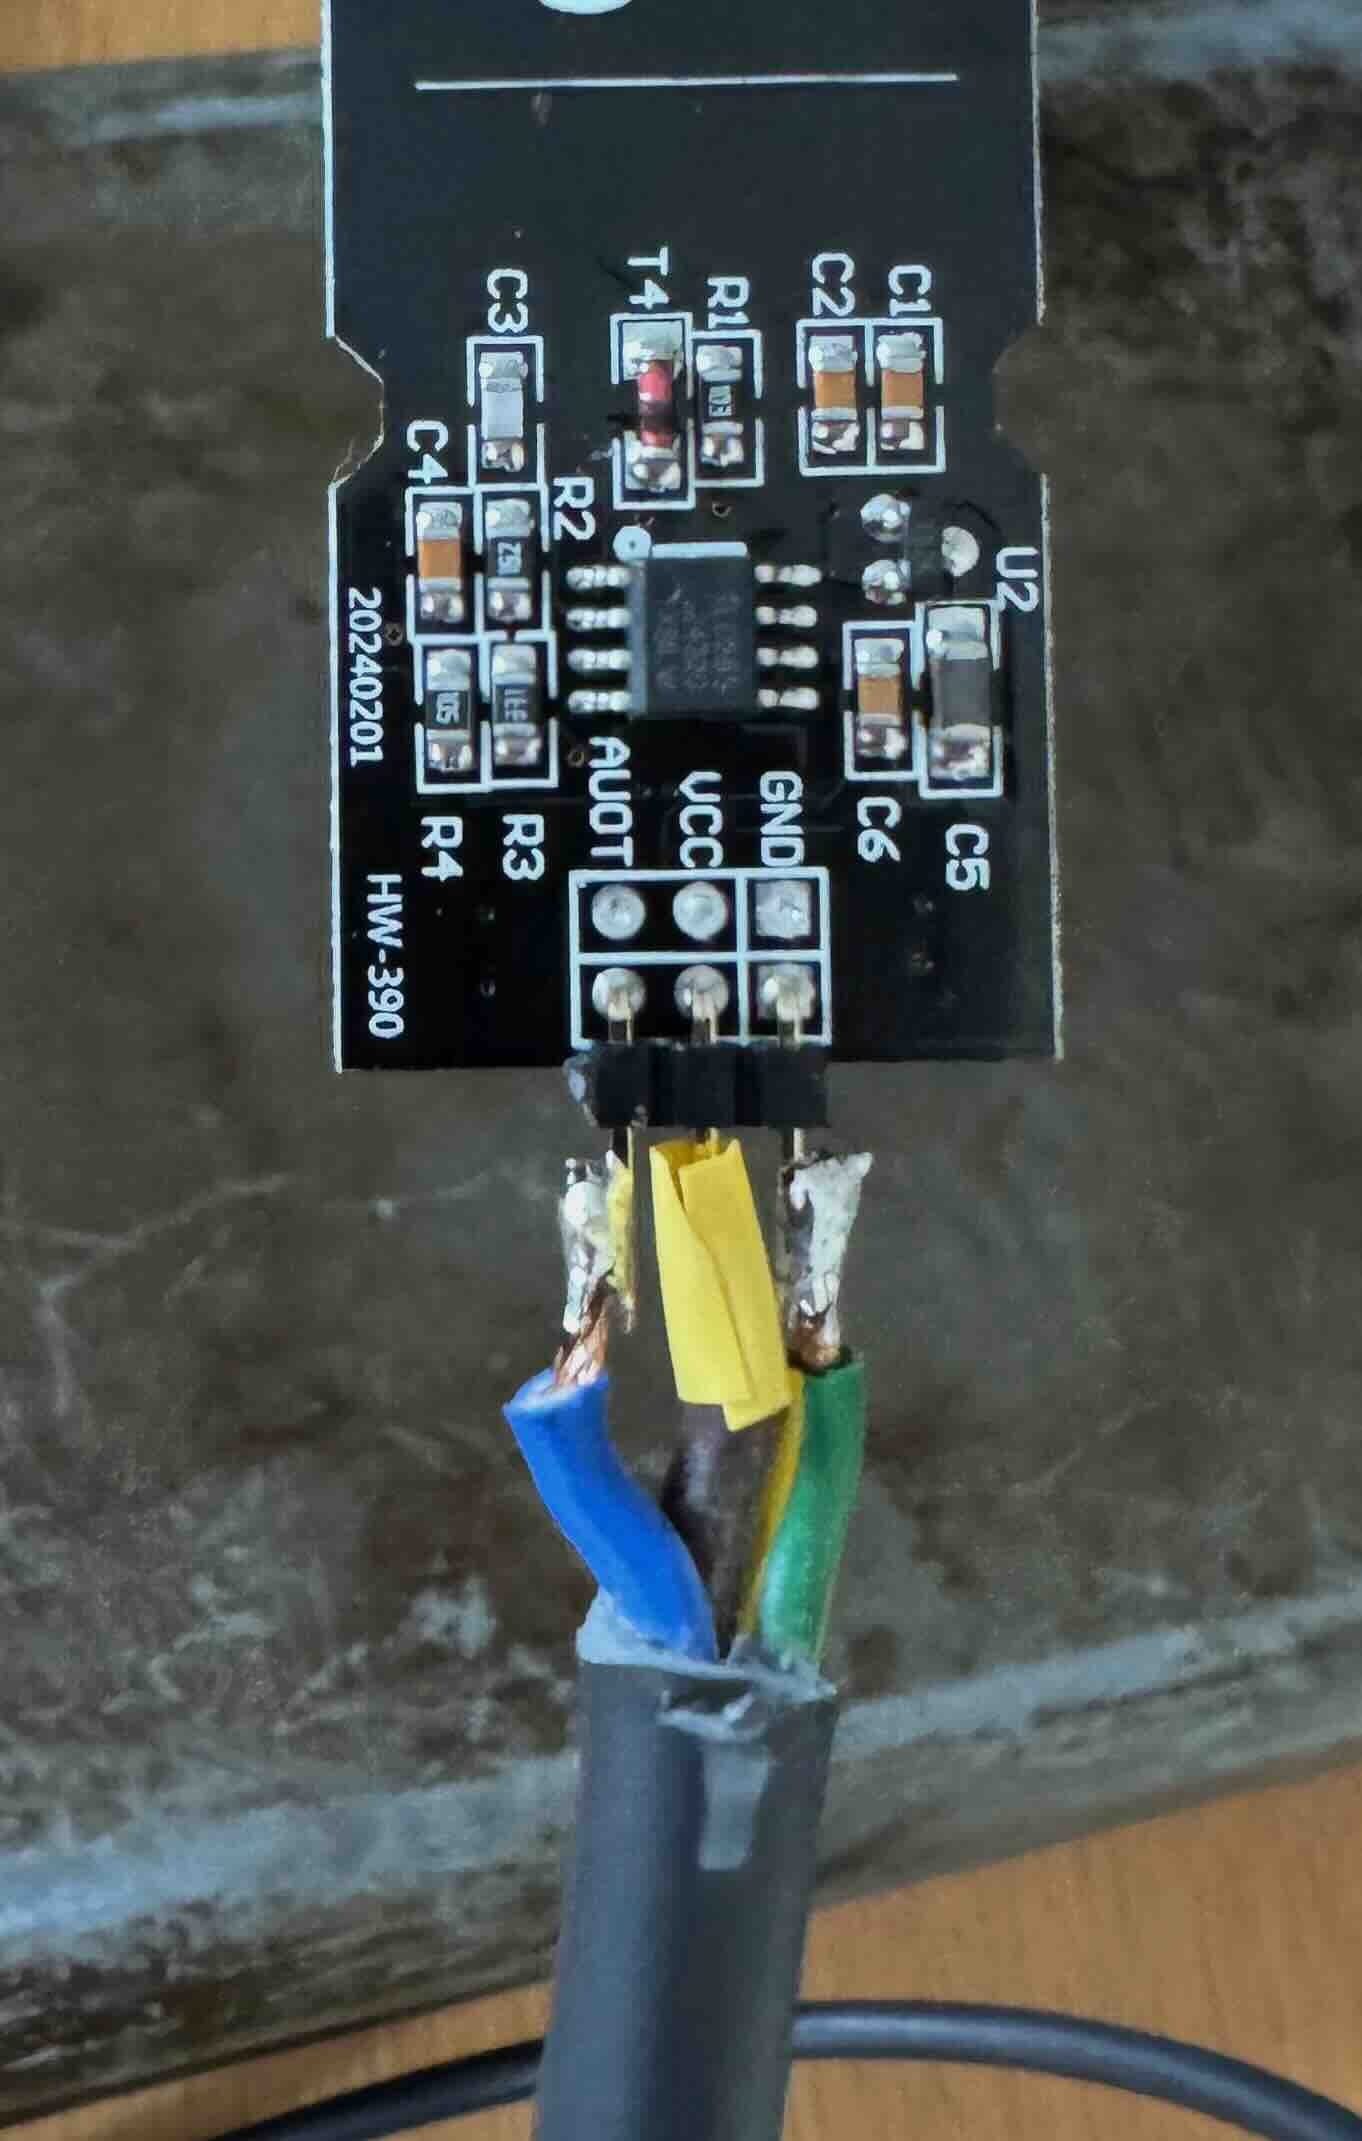
\includegraphics[width=0.3\textwidth]{contents/part-2/fig2/solder-soil.jpeg}
    \caption{Soldered soil moisture sensor}
    \label{fig:solder-soil}
\end{figure}

Waterproofing the sensor was necessary as while the bottom three quarters of the
board are designed to be inserted into soil, the part above this is made up of
exposed electronics that cannot contact water (Refer to figure
~\ref{fig:soil-sensor}). This means this part of the board would be directly
exposed to the elements unless waterproofing is applied

To waterproof this sensor I followed an online tutorial on a hobbyist website
\cite{waterproof-sensor}. The method involves painting the electronics using
nail varnish, while this sounds unconventional, nail varnish is a non-conductive
compound that can be easily painted over electronics with the included brush. It
is therefore quite a popular low-cost method for waterproofing electronics.
After this is applied the portion of the board with the electronics is covered
in heatshrink to form a tight seal over the board, with a layer of nail polish
on the edges to reduces the chance of water ingress under the heat shrink's
plastic.

ADD FIGURE HERE

\subsubsection{Other external components}

The DHT11 sensor was mounted inside a smaller IP55-rated junction box, which
provides the same resistance against rain as the larger box. To allow for more
accurate readings, small holes were drilled on the bottom panel of this so the
air temperature inside the box would better match the external
temperature/humidity. To further improve the sensor's accuracy, the box was
painted white to reflect sunlight, and a solar shield made from a cut and
reshaped aluminium can was mounted to the south facing side. This shield helps
to prevent direct sunlight exposure to the sensor, reducing temperature
distortion while still allowing airflow from the sides.

The solar panel was mounted below the main enclosure using the included
adjustable gimbal mount. It was fixed at an angle of approximately 40° from
horizontal, which balances solar efficiency throughout the year. This angle is
steeper than the optimal summer setting but allows for improved performance
during winter months when the sun is lower in the sky. The gimble allows for
rotation in all planes which is useful in case the box itself cannot be mounted
in a perfect south direction. 

The anemometer was secured to a separate length of wood, positioned
approximately 0.5 metres away from the main unit. This separation reduces
turbulence caused by the box and pole, leading to more accurate wind speed
readings. The sensor was screwed directly into the wood and positioned at a
height of 2m.

ADD final assembled box on a pole with annotations

\subsubsection{Gateway}

The gateway node required less careful engineering as there was no requirement
for it to be waterproofed or mounted externally. As this would eventually be
placed inside a persons private home, the aim was therefore to make a minimally
imposing and so a design similar to an internet router was chosen.

The two devices inside the box would be the raspberry pi used to upload data and
the challenger which received incoming LoRa packets from the repeater. A plastic
box was used with cut outs for the pi's outputs and power cable, with an
additional cut out on the lid for the challenger's antenna. The pi and
challenger were then secured to the box's base with velcro tape, as both devices
would potentially need to be removed for any trouble shooting.